\newpage
\section{Aufgabe2}
\label{sec:a2}

\subsection{a)}
\label{subsec:a2a}
In der Abbildung \ref{fig:scatter} sind die beiden Populationen
$P0$ und $P1$ sowie die drei Projektionsgeraden:
\begin{align}
  g_1(x)=0\\
  g_2(x)=-\frac34x\\
  g_3(x)=-\frac54x
\end{align}
\begin{figure}
  \centering
  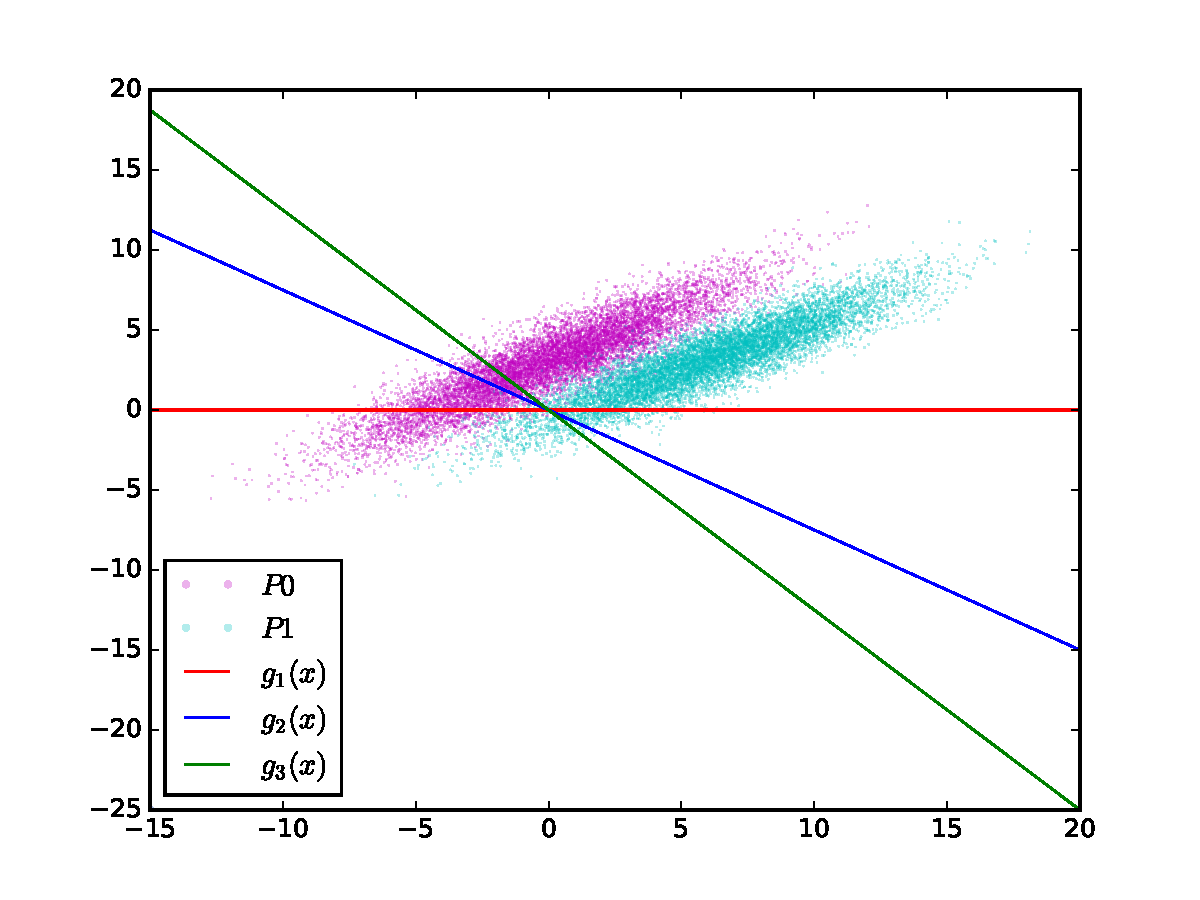
\includegraphics[width=0.7\textwidth]{scatterplot2D.pdf}
  \caption{Zweidimensionaler Scatterplot der Populationen und die
  Projektionsgeraden.}
  \label{fig:scatter}
\end{figure}

\subsection{b)}
\label{subsec:a2b}
Um die Populationen $P0$ und $P1$ jeweils auf die Geraden zu
projezieren, muss zu nächst der Richtungsvektor
der Geraden bestimmt
und normiert werden.
\paragraph{Richtungsvektor $g_1(x)$:}
\begin{align}
\vec v_1 =
\begin{pmatrix}
   1\\
   0
\end{pmatrix}.
\end{align}
Dieser Vektor ist schon normiert, folglich muss nur noch die
Richtung umgedreht werden damit die projizierte Population $P0$
rechts
von der Population $P1$ liegt.
\begin{align}
  \Rightarrow \v_1=
  \begin{pmatrix*}[r]
     -1\\
     0
  \end{pmatrix*}
\end{align}

\paragraph{Richtungsvektor $g_2(x)$:}
\begin{align}
\vec v_2 =
\begin{pmatrix*}[r]
   1\\
   -\frac{3}{4}
\end{pmatrix*}.
\intertext{Normierung:}
\left|n\cdot
\begin{pmatrix*}[r]
    1\\
  -\frac{3}{4}
\end{pmatrix*}
\right|&\stackrel{!}{=} 1\\
n\sqrt{1^2+\left(\frac34\right)^2}&\stackrel{!}{=} 1\\
n&=\frac45\\
\Rightarrow \vec v_2=
\begin{pmatrix*}[r]
    \frac45\\
  -\frac{6}{10}
\end{pmatrix*}
\intertext{Wegen der Reihenfolge muss der Vektor wieder umgedreht werden.}
\Rightarrow \vec v_2=
\begin{pmatrix*}[r]
  -\frac45\\
  \frac{6}{10}
\end{pmatrix*}
\end{align}


\paragraph{Richtungsvektor $g_3(x)$:}
\begin{align}
\vec v_3 =
\begin{pmatrix*}[r]
   1\\
   -\frac{5}{4}
\end{pmatrix*}.
\intertext{Normierung:}
\left|n\cdot
\begin{pmatrix*}[r]
    1\\
  -\frac{5}{4}
\end{pmatrix*}
\right|&\stackrel{!}{=} 1\\
n\sqrt{1^2+\left(\frac54\right)^2}&\stackrel{!}{=} 1\\
n&=\frac4{\sqrt{41}}\\
\Rightarrow \vec v_3=
\begin{pmatrix*}[r]
    \frac4{\sqrt{41}}\\
  -\frac{5\sqrt{41}}{41}
\end{pmatrix*}
\intertext{Wegen der Reihenfolge muss der Vektor wieder umgedreht werden.}
\Rightarrow \vec v_3=
\begin{pmatrix*}[r]
    -\frac4{\sqrt{41}}\\
  \frac{5\sqrt{41}}{41}
\end{pmatrix*}\end{align}
\paragraph{Projektionen}
In den Abbildungen \ref{fig:histg1}-\ref{fig:histg3} sind
die eindimensionalen Histogramme der Projetktionen
auf die jeweiligen
geraden zu  finden.
Die Projektion der Punkte auf die Gerade $g_i$ der Population wird mit Hilfe
der Formel
\begin{align}
  x=\vec v_i^\top \cdot \vec x
\end{align}
berechnet.

\begin{figure}
  \centering
  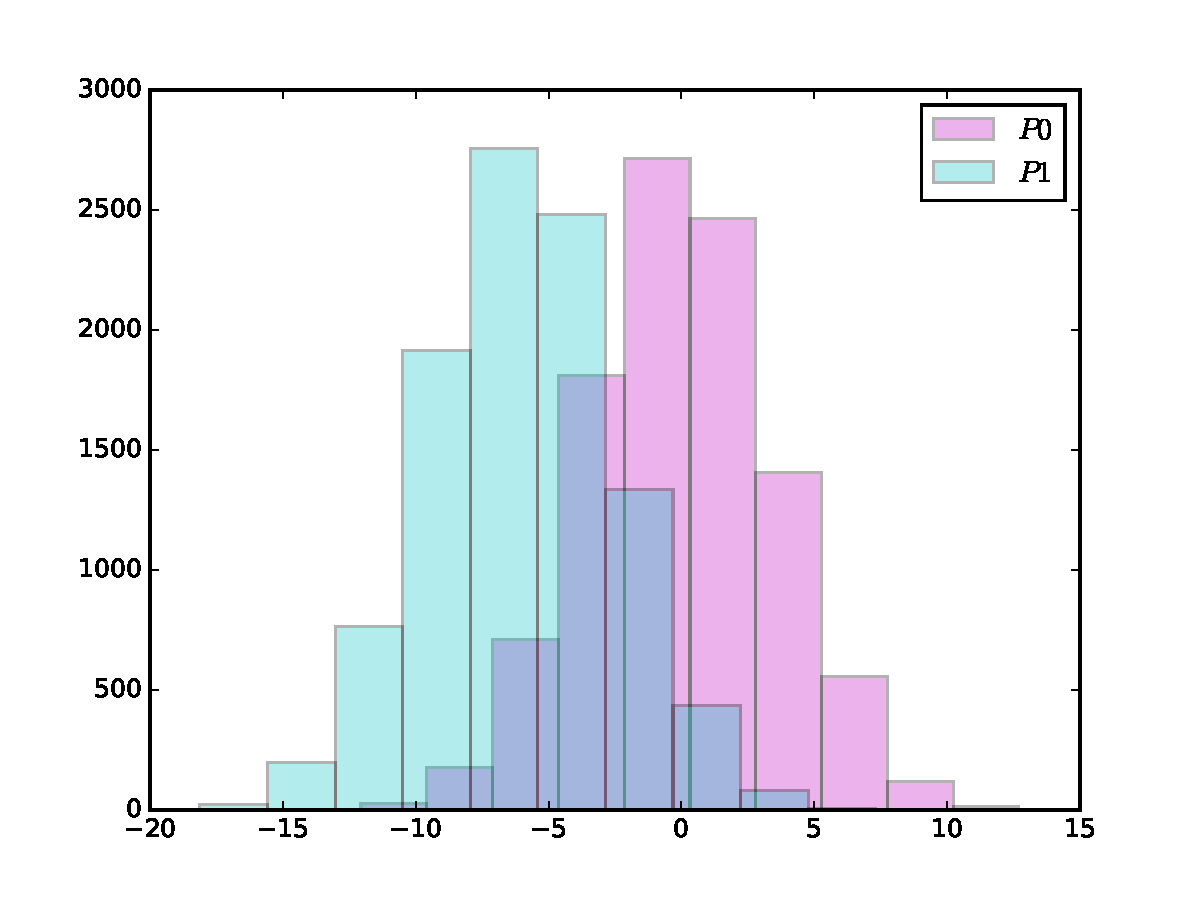
\includegraphics[width=0.7\textwidth]{g_1.pdf}
  \caption{Histogramm der Projektion
   von den Populationen $P0$ und $P1$ auf die Projektionsgeraden $g_1(x)$.}
  \label{fig:histg1}
\end{figure}


\begin{figure}
  \centering
  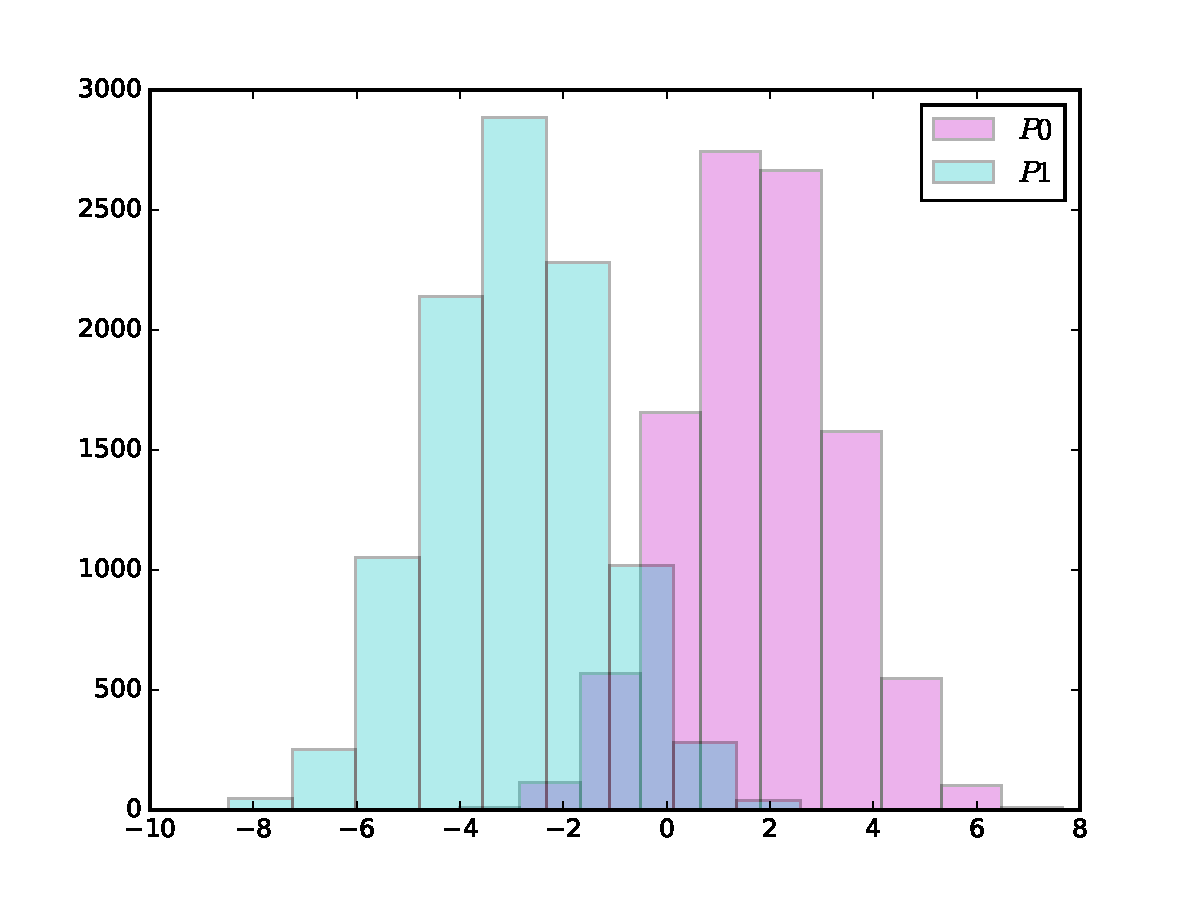
\includegraphics[width=0.7\textwidth]{g_2.pdf}
  \caption{Histogramm der Projektion
   von den Populationen $P0$ und $P1$ auf die Projektionsgeraden $g_2(x)$.}
  \label{fig:histg2}
\end{figure}


\begin{figure}
  \centering
  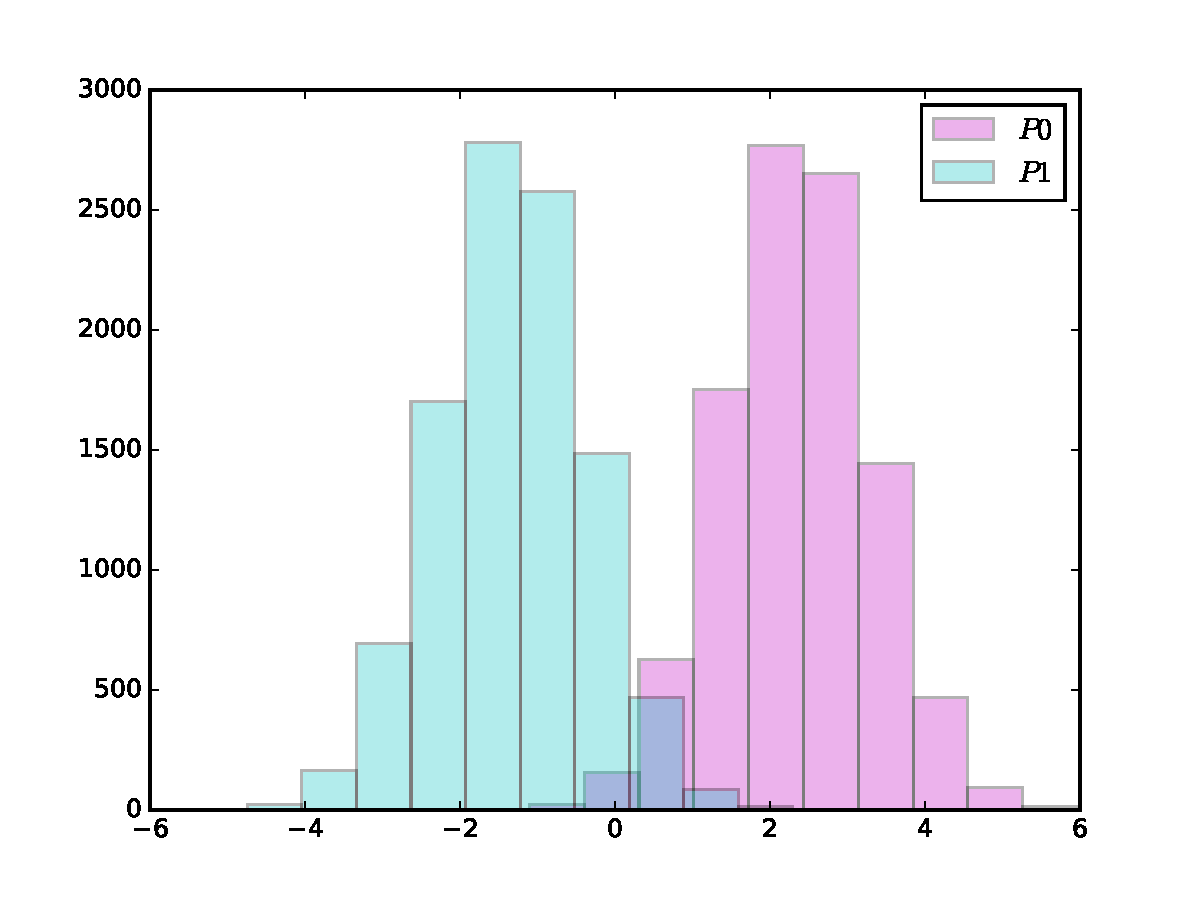
\includegraphics[width=0.7\textwidth]{g_3.pdf}
  \caption{Histogramm der Projektion
   von den Populationen $P0$ und $P1$ auf die Projektionsgeraden $g_3(x)$.}
  \label{fig:histg3}
\end{figure}






\subsection{c)}
\label{subsec:a2c}
Betrachtet man nun $P0$ als Signal und $P1$ als Untergrund kann die
Effizienz und Reinheit des Signals als Funktion eines Schnitts
$\lambda_\mathrm{cut}$ aufgetragen werden.
Die jeweiligen Plotts sind in den Abbildungen \ref{fig:cut1} -\ref{fig:cut3}
dargestellt.

\begin{figure}
  \centering
  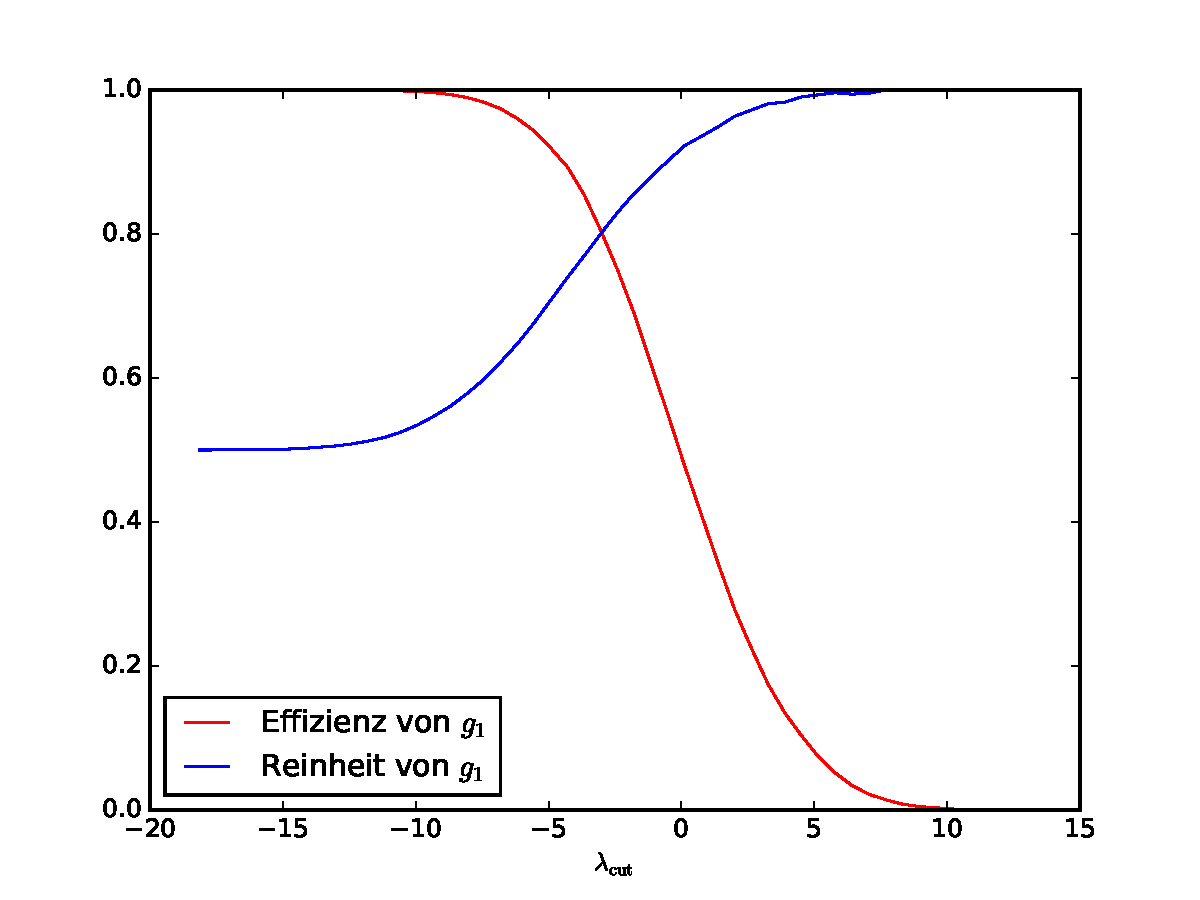
\includegraphics[width=0.7\textwidth]{g_1Effizienz.pdf}
  \caption{Effizienz und Reinheit des Schnittes ausgehend von der Gerade $g_1$ in Abhängigkeit von $\lambda_\text{cut}$ .}
  \label{fig:cut1}
\end{figure}



\begin{figure}
  \centering
  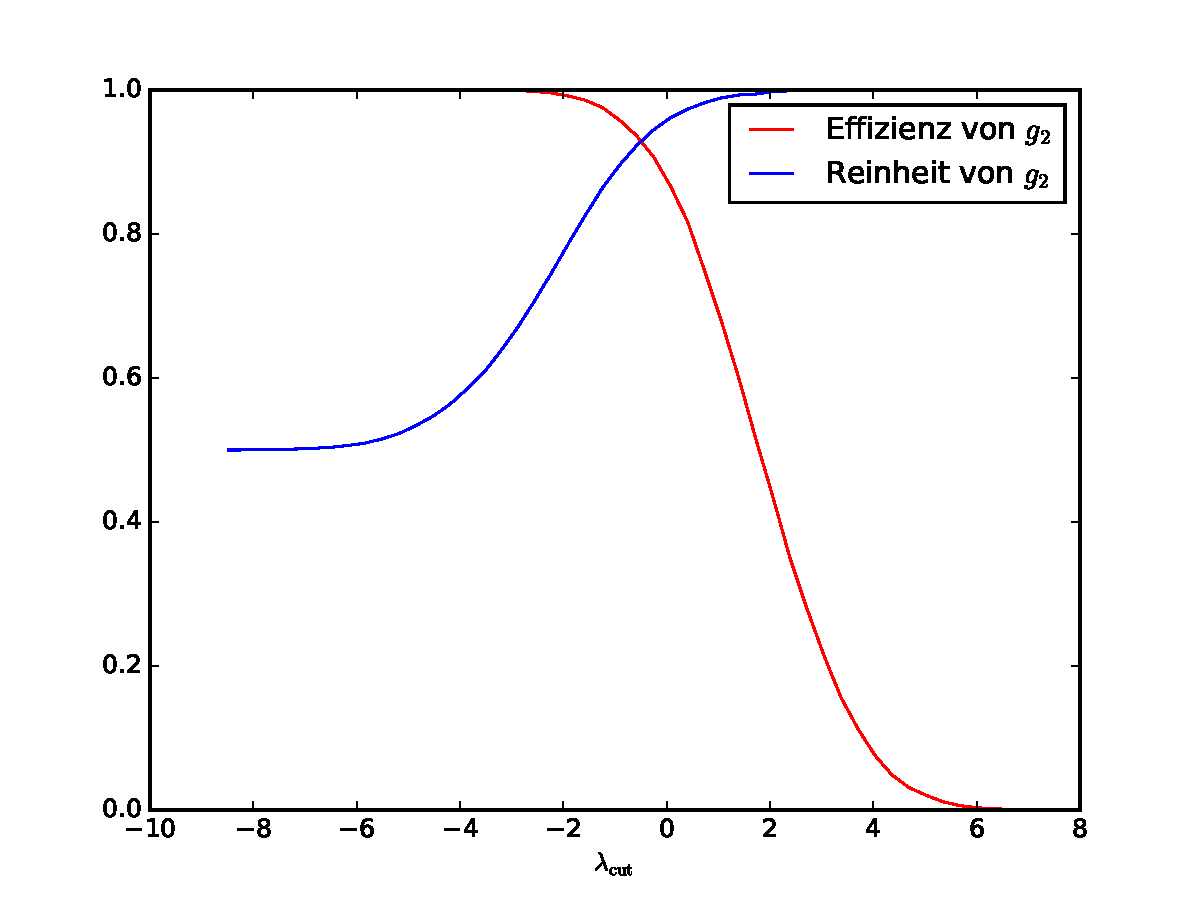
\includegraphics[width=0.7\textwidth]{g_2Effizienz.pdf}
  \caption{Effizienz und Reinheit des Schnittes ausgehend von der Gerade $g_2$ in Abhängigkeit von $\lambda_\text{cut}$ .}
  \label{fig:cut2}
\end{figure}



\begin{figure}
  \centering
  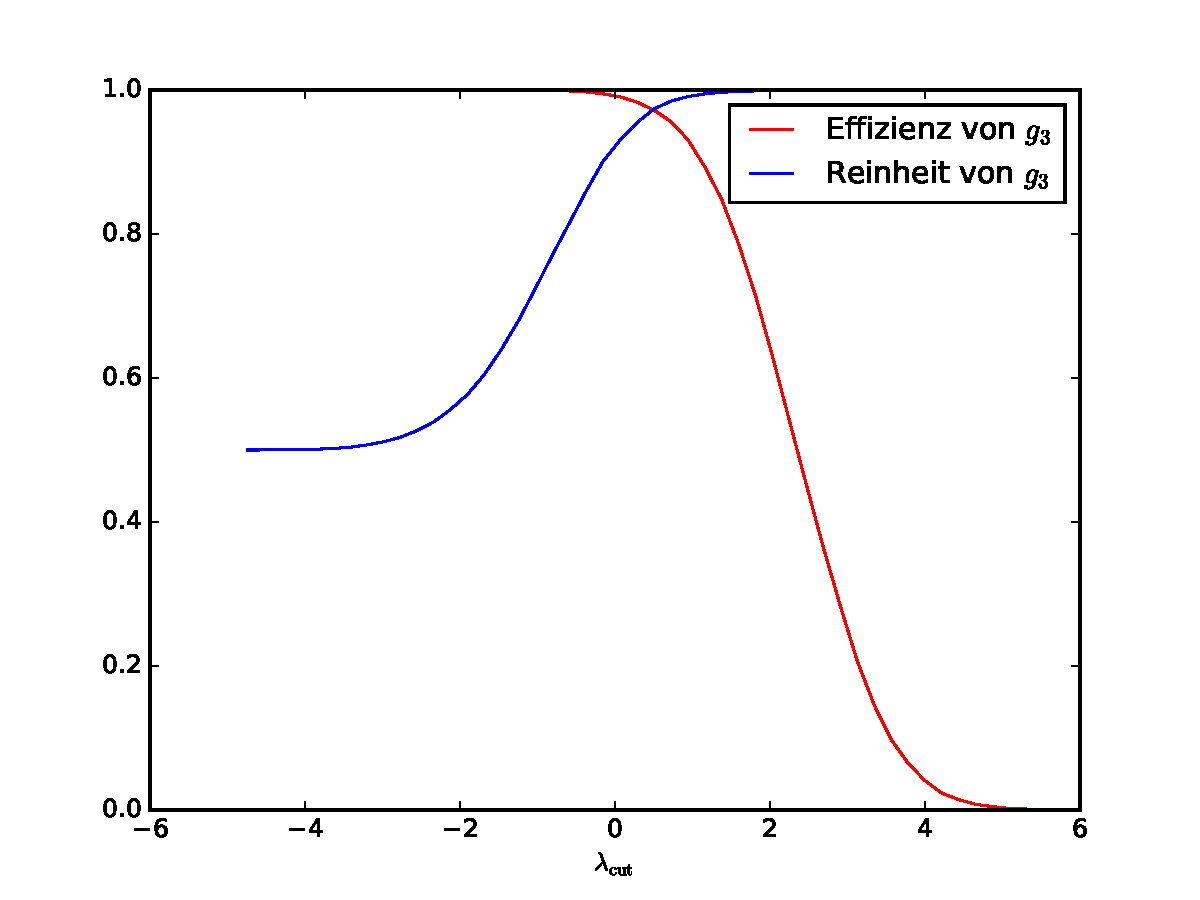
\includegraphics[width=0.7\textwidth]{g_3Effizienz.pdf}
  \caption{Effizienz und Reinheit des Schnittes ausgehend von der Gerade $g_3$ in Abhängigkeit von $\lambda_\text{cut}$ .}
  \label{fig:cut3}
\end{figure}
